\section{Computational aspects}
\label{Sec2:compAsp}
\tikzstyle{startstop} = [rectangle, minimum width=3cm, minimum height=1cm,text centered, draw=black, fill=yellow!30]
\tikzstyle{forloopbegin} = [rectangle, minimum width=5cm, rounded corners, minimum height=1cm, text centered, text width=5cm, draw=black, fill=green!30]
\tikzstyle{forloopend} = [circle, draw=black, fill=green!30]
\tikzstyle{processPar} = [text width=5cm, rectangle, rounded corners, minimum width=1cm, minimum height=1cm, text centered, draw=black, fill=blue!30]
\tikzstyle{process} = [rectangle, minimum width=5cm, minimum height=1cm, text centered, text width=5cm, draw=black, fill=blue!30]
\tikzsetnextfilename{flowchart} 
\begin{figure}
	\centering
	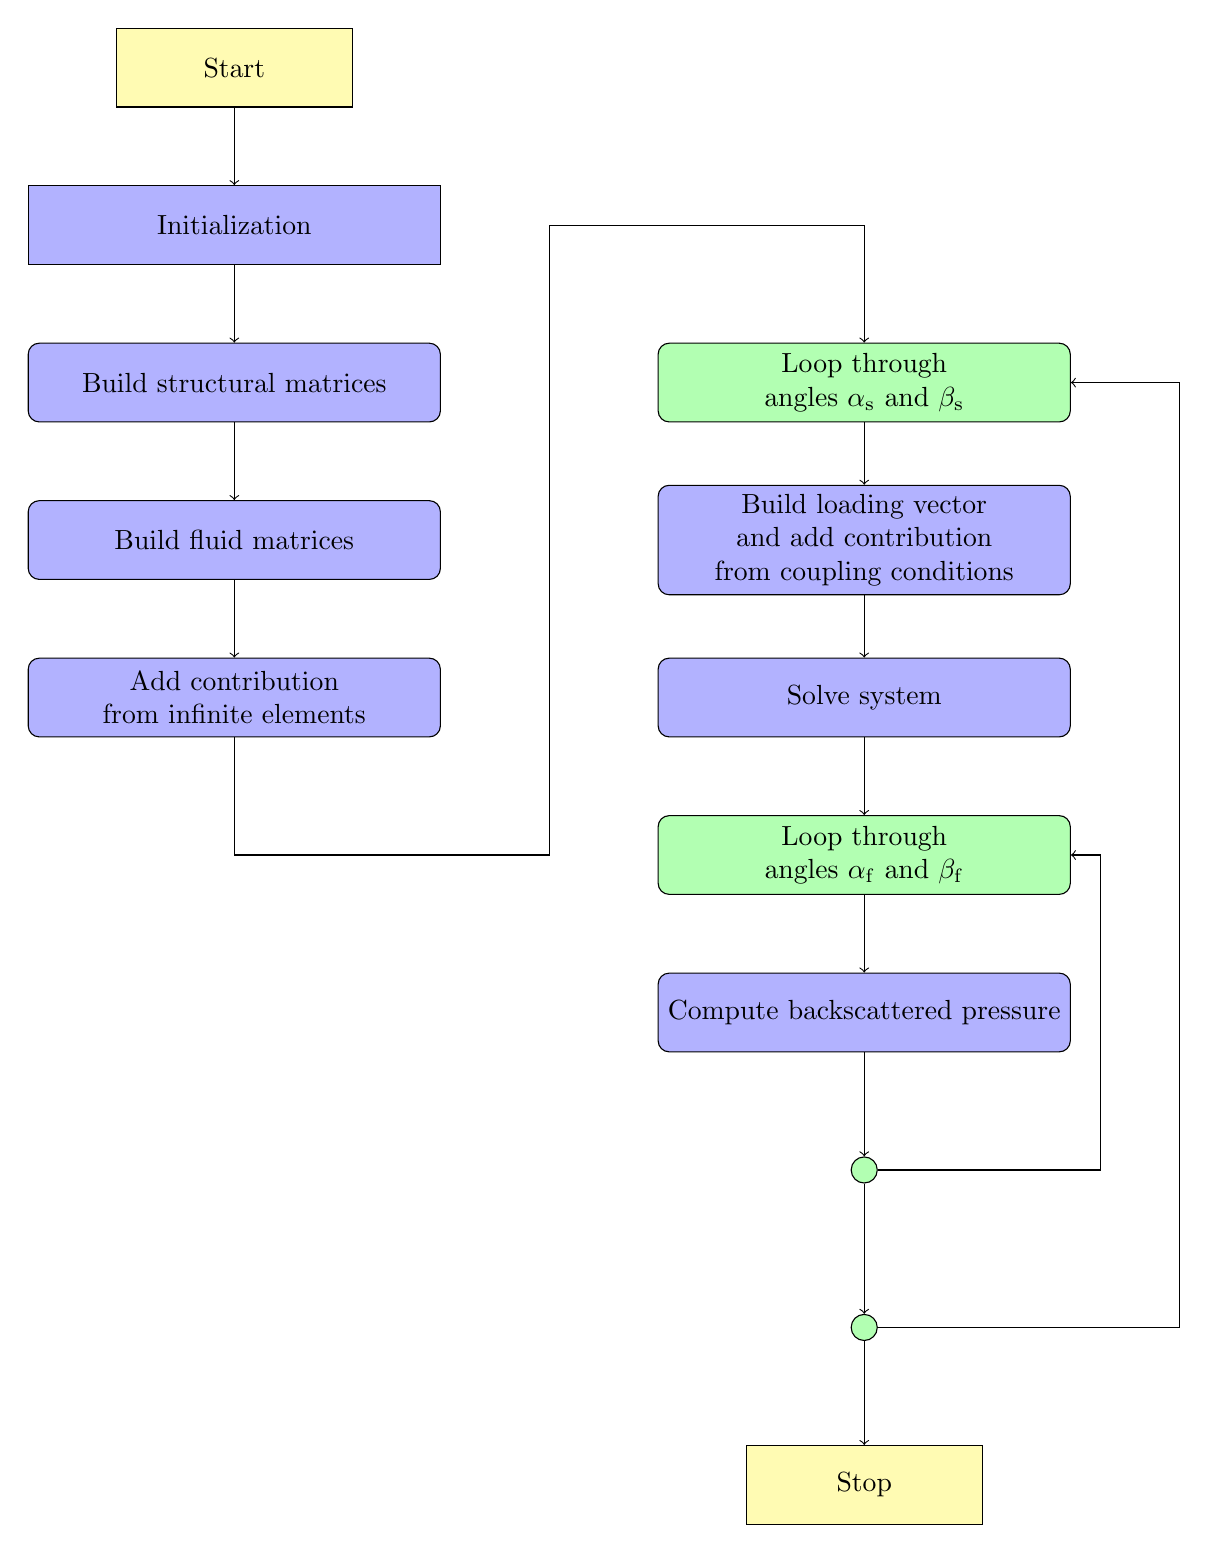
\begin{tikzpicture}[node distance=2cm]

	\node (start) [startstop] {Start};
	\node (NURBS) [process, below of=start] {Initialization};
	\node (structure) [processPar, below of=NURBS] {Build structural matrices};
	\node (fluid) [processPar, below of=structure] {Build fluid matrices};
	\node (infelems) [processPar, below of=fluid] {Add contribution from infinite elements};
	\node (ghost1a) [below of=infelems] {};
	\node (ghost1b) [right of=ghost1a, xshift=2cm] {};
	\node (ghost1c) [right of=NURBS, xshift=2cm] {};
	\node (ghost1d) [right of=ghost1c, xshift=2cm] {};
	
	\node (loopLoading) [forloopbegin, below of=ghost1d] {Loop through \\ angles $\alpha_{\mathrm{s}}$ and $\beta_{\mathrm{s}}$};
	\node (ghost2a) [right of=loopLoading, xshift=2cm] {};
	\node (loading) [processPar, below of=loopLoading] {Build loading vector and add contribution from coupling conditions};
	\node (solveSystem) [processPar, below of=loading] {Solve system};
	
	\node (loopFarField) [forloopbegin, below of=solveSystem] {Loop through \\ angles $\alpha_{\mathrm{f}}$ and $\beta_{\mathrm{f}}$};
	\node (ghost3a) [right of=loopFarField, xshift=1cm] {};	
	\node (farField) [processPar, below of=loopFarField] {Compute backscattered pressure};
	\node (forloopfinishFarField) [forloopend, below of=farField] {};
	\node (ghost3b) [right of=forloopfinishFarField, xshift=1cm] {};	
	\node (forloopfinishLoading) [forloopend, below of=forloopfinishFarField] {};
	\node (ghost2b) [right of=forloopfinishLoading, xshift=2cm] {};
	\node (stop) [startstop, below of=forloopfinishLoading] {Stop};
	
	\draw [->] (start) -- (NURBS);
	\draw [->] (NURBS) -- (structure);
	\draw [->] (structure) -- (fluid);
	\draw [->] (fluid) -- (infelems);
	\draw [->] (infelems) |- (ghost1b) -- (ghost1a) -| (ghost1c) -- (ghost1b)  |- (ghost1d) -- (ghost1c) -| (loopLoading);
	
	\draw [->] (loopLoading) -- (loading);
	\draw [->] (loading) -- (solveSystem);
	\draw [->] (solveSystem) -- (loopFarField);
	\draw [->] (loopFarField) -- (farField);
	\draw [->] (farField) -- (forloopfinishFarField);
	\draw [->] (forloopfinishFarField) -- (forloopfinishLoading);
	\draw [->] (forloopfinishFarField) -| (ghost3a) -- (ghost3b) |- (loopFarField);
	\draw [->] (forloopfinishLoading) -| (ghost2a) -- (ghost2b) |- (loopLoading);
	\draw [->] (forloopfinishLoading) -- (stop);
	
	
	\end{tikzpicture}
	\caption[The flowchart of the full FSI program]{\textbf{The FSI program}: The flowchart of the full FSI program analyzing both monostatic and bistatic cases. The boxes with rounded corners are parallelized.}
	\label{Fig2:flowchart}
\end{figure}
In \Cref{Fig2:flowchart} we give an overview of the code for the full fluid structure interaction program for both monostatic and bistatic cases. The only part which is not parallelized is the initialization part of the code. The time elapsed by this part is negligible in comparison with any other part of the program, so any effort for optimizing this part was omitted. In the following we shall briefly present the main content of each step.

\subsection{Initialization}
The initialization part consist of defining all relevant parameters and constructing the mesh for analysis. To create the IGA mesh, we first import data for the coarsest mesh of the NURBS object (i.e. data set's found in \Cref{Sec2:NURBSdata}). One typically first constructs the NURBS object for the solid domain as this domain should be the exact representation of the given object. In contrast, we have more degrees of freedom when construction the fluid mesh. The mesh for the fluid domain must be constructed by finding a suitable spheroid which may be wrapped closely around the obstacle without creating to much of a distortion in the resulting mesh (see \Cref{subse:ConstructionModel3Mesh}). Although it may certainly be possible, it has not been implemented an automated algorithm for finding such a spheroid. So in the analysis, we have found the fluid mesh by trial and failure. When the two meshes have been constructed (two NURBS patches) one has many opportunities of $k$-refinement. The two algorithms \mcode{elevateNURBSdegree} and \mcode{insertKnotsInNURBS} have been implemented for this purpose (see \Cref{subse:NURBSvolumes}). Typically we order elevate first to the desired degrees in $\xi$-, $\eta$- and $\zeta$-direction. Then we insert the desired number of knots in the desired locations (creating more elements for analysis). From this point, we are able to create the IGA mesh. We first construct an ordering of the available NURBS basis functions, then we construct a connectivity array which for each element links every basis functions having support on this element. From here, it is important to have knowledge if there is any periodicity involved for the NURBS patch. If this is the case, one must find the overlapping control points causing the periodicity. There could potentially be more than two control points at the same physical location. In any case, define the control point with lowest index to be the ``parent function'' and the rest ``children functions''. Then one constructs an array mapping all children functions to the parent function. This array is then used to modify the mentioned connectivity array. In addition to keeping track of the indices for the parent functions, one must also store the indices for the children functions as these degrees of freedom must be removed from the global system matrix.

\subsection{Structural matrices and fluid matrices}
When constructing the stiffness matrix and the mass matrix, we create four arrays for these two matrices. The first two arrays will contain the indices (columns and rows) in the global matrix. The other two arrays stores the contribution at these indices for each of the two matrices. We continue by creating an array of Gaussian quadrature points and weights. The code supports 64 Gaussian quadrature points per direction such that one is able to evaluate a 3D IGA element at $64^3=262144$ points. However, one typically determines the number of control points by the NURBS degree for each of the parameter directions. More specifically, if the degree in $\xi$ direction is $p$, then we use $p+1$ quadrature points in this direction. Thus, we have $(p+1)(q+1)(r+1)$ quadrature points per volume element. 

It is very important to note that the global stiffness matrix is very sparse. Not only is it a huge advantage in \MATLAB to have the matrix in sparse format when solving the linear system, but also when assembling the matrix. If the matrix is made sparse only after assembly, then the initialization would require \MATLAB to allocated place for a full stiffness matrix. This is very memory consuming and should be avoided if one wants to run the program with many degrees of freedom. A matrix in sparse format contains 3 columns; the first two represent the indices in the matrix and the third column represent the corresponding value. The problem of preallocation may be solved by first construct these three columns in three arrays. By noting that each element stiffness matrix has $\left[3(p+1)(q+1)(r+1)\right]^2$ number of components, we initialize the arrays by the following.
\begin{lstlisting}
n_en = (p+1)*(q+1)*(r+1);
sizeOfk_e = (3*n_en)^2;
indices = zeros(3*n_en,noElems); 
spIdxRow = zeros(sizeOfk_e,noElems);
spIdxCol = zeros(sizeOfk_e,noElems);
Kvalues = zeros(sizeOfk_e,noElems); 
\end{lstlisting}
Note that we initialize these ``vectors'' in matrix form as this allows us to easily parallelize using \mcode{parfor} in \MATLAB.

Note that we do not here sum overlapping element matrices, but this is automatically done when the \mcode{sparse} function is called in \MATLAB.
\begin{lstlisting}
K = sparse(spIdxRow,spIdxCol,values);
\end{lstlisting}
That is, there will be index combinations which will repeat and therefore this method would require a lot more memory. Using server with 256GB memory space, one is able to run this implementation with up to $10^6$ degrees of freedom, which is more than enough for this thesis. Thus, the results evaluated for this thesis is done relatively fast.

The other obvious method is simply using
\begin{lstlisting}
K(sctrB,sctrB) = K(sctrB,sctrB) + k_e;
\end{lstlisting}
which typically results in the \MATLAB warning ``This sparse indexing expression is likely to be slow''. In~\cite{Karatarakis2013cot} it is described how one could optimize the assembly, and in~\cite{Hughes2010eqf} we find theory around efficiently use of quadrature for NURBS. In~\cite{Jansson2013osm} a new stack based representation of the sparse matrix is presented, which could speed up the matrix assembly part. This is however outside the scope of this thesis, and is therefore not included.

We are now ready to loop through all structure elements and calculate their contribution to the stiffness and mass matrix. For each element in this loop (which is parallelized) we must loop through all quadrature points. For each quadrature point in this inner loop, we evaluate all the NURBS basis functions which have support on the current element. The Jacobian is then computed (by \Cref{Eq2:NURBSjacobian}) in order to find the derivative of the basis functions with respect to physical coordinates (\Cref{Eq2:basisFunsDerivativeRel}) which is then used to find the strain matrix $\vec{B}$ (\Cref{Eq2:strainMatrixB}). Note that if body forces is to be applied to the solid, these will be calculated in this same loop. So one must not mistake the part of building the loading vector with the implementation of body forces. However, we never encounter body forces in the analysis of acoustic scattering, but it has been implemented anyways as some static elasticity problems involving body forces has been analyzed in this thesis (the Kneaded cylinder in \Cref{subse:KneadedCylinder} and Scordelis-Lo Roof in \Cref{subse:Scordeli}).

After looping through all elements, one creates the sparse matrices $\vec{K}$ and $\vec{M}$ using the \mcode{sparse} function in \MATLAB. These matrices are then added (with a scaling factor for the mass matrix). The reason why they are not added during calculation is simply to create a more general function which handles the elastostatic case as well (no construction of the mass matrix).

The next step is to construct the matrices for the fluid part of the domain. The setup is almost identical to the case for the structure matrices. However, we are now working with scalar valued domain instead of a vector valued domain. This will affect the indexing. In addition, the bilinear form is different for the two cases. After computing the fluid matrices, the result is added to the global matrix.

\subsection{Contribution from infinite elements}
The infinite elements are implemented using the multi-pole expansion after Burnett in~\cite{Burnett1994atd}. We generalize this work, which was based on the BGU formulation, to the other three formulations BGC, PGU and PGC (see \Cref{se:infElems}).

One first needs to locate the indices for the NURBS basis functions having support on the artificial boundary $\Gamma_{\mathrm{a}}$. In addition, the radial integrals in the bilinear or sesquilinear form must be computed (depending on which infinite element formulation is chosen). Finally, one must compute the coefficients used for the radial basis functions in the infinite elements (from the relation \Cref{Eq2:infElemCoeffs}). These two last step suffers from round off errors for a high number of infinite element radial basis functions $N$. The way to solve this is to increase the precision using the mentioned MuPAD in \MATLAB.

We are now ready to loop through all surface elements on $\Gamma_{\mathrm{a}}$. Once again, for each element, we have an inner loop over all quadrature points. And for each quadrature points, the NURBS basis functions are evaluated, such that the Jacobi matrix can be computed. This is in turn used to compute the derivative with respect to the prolate spheroidal coordinates. In this regards it has been implemented a function which evaluates $(r,\vartheta,\phi)$ for a given point $(x,y,z)$ (using the relations in \Cref{Eq2:XtoProl}). Moreover, the derivatives of $(r,\vartheta,\phi)$ with respect to $(x,y,z)$ must be computed (using the relations in \Cref{Eq2:dProlateSphericalCoordinatesdX}). We may then compute the derivatives of $(r,\vartheta,\phi)$ w.r.t, the surface parameters $\xi$ and $\eta$ using \Cref{Eq2:dPdNURBS}. These derivatives are finally used to evaluate the derivatives of the basis functions with respect to the angles $\vartheta$ and $\phi$ using \Cref{Eq2:dRdP}. This enables us to compute the contributions to the surface integrals $J_{AB}^{(1)}$, $J_{AB}^{(2)}$, $J_{AB}^{(3)}$, $J_{AB}^{(4)}$ and $J_{AB}^{(5)}$ (expressions in \Cref{Eq2:surfaceIntegralsInfElems}). Note that we do not compute the full bilinear or sesquilinear form in this inner loop, as the radial integrals is independent of the angular coordinates (to avoid redundant computations). After looping through the quadrature points, we continue the loop on the current element and evaluates the bilinear or the sesquilinear form. This is done by looping through all radial basis functions in the infinite elements. The result is then collected and added to the global matrix.

\subsection{Loading vector and coupling condition}
The coupling conditions connects the two spaces for the solid domain and the fluid domain. This involves a coupling of two NURBS objects. The implementations assume the surfaces to be connected have the same NURBS parametrization. It also assumes the NURBS patches to be parametrized in such a way that these surfaces are given at $\zeta=0$ for the fluid and $\zeta =1$ for the solid. This causes restriction in the refinement process; if we want to, say, insert a knot in the $\xi$ direction, or order elevate in this direction in the fluid, we must do the same refinement process in the solid.

Keeping these remarks in mind, we start again by constructing the surface mesh. This mesh is constructed on the basis of the surface at $\zeta=1$ for the solid. We then loop through these surface elements, and for each element we must loop through the quadrature points. For each such quadrature point we now evaluate 2D NURBS functions, as we know the 3D NURBS functions reduce to 2D NURBS functions when $\zeta$ is constant. This obviously saves a lot of computations. Once again, these evaluations are used to compute the (2D) Jacobian which is in this case not used to evaluate derivatives of the NURBS functions w.r.t. physical coordinates, as they do not appear in the coupling conditions. The Jacobian is only used to compute the cross product needed to compute the surface integral (see \Cref{Eq2:surfIntegral}). This cross product is also needed to determine the normal vector in the coupling term in the FSI bilinear form (\Cref{Eq2:FSIbilinearForm}). As we want this normal vector to point out from the solid domain, and we consider the NURBS parametrization of the solid domain, the normal vector is given by
\begin{equation*}
	\vec{n} = \frac{\pderiv{\vec{X}}{\xi}\times\pderiv{\vec{X}}{\eta}}{\left\| \pderiv{\vec{X}}{\xi}\times\pderiv{\vec{X}}{\eta}\right\|}
\end{equation*}
for right hand oriented NURBS parametrization. It is here assumed that the parametrization is orientable. The parametrization is right hand oriented whenever $\det(\vec{J})>0$ throughout the domain. If $\det(\vec{J})<0$ throughout the domain, we simply need to change the sign of the normal vector in the expression above.

We continue by computing the physical coordinates in order to evaluate the given incident field $p_{\mathrm{inc}}$ and its derivative. The result is then collected and added to the global matrix. Note that the other contributions to the global matrix is independent of the incident field such that they only need to be computed once (thus we store this part). Moreover, if only hard walled boundary conditions are considered (only fluid, and no coupling), then there is no update in the global matrix in this loop. If a direct solver is chosen, one may split the loop over the angles $\alpha_{\mathrm{s}}$ and $\beta_{\mathrm{s}}$ such that the factorization is only done once. 

\subsection{Solving the system}
If there are many angles to be analyzed, the loops over these angles should be parallelized. However, if one only consider few angles (for instance the bistatic case when only one pair of $\alpha_{\mathrm{s}}$ and $\beta_{\mathrm{s}}$ is considered), one should take the parallelization over the loop which runs through the surface elements.

When a direct solver is to be used, the backslash operator in \MATLAB will elegantly solve the problem in a efficient way. However, if the LU factorization may be reused (which is the case when no coupling is present) one should use the build in \mcode{lu} function. If the LU factorization is reused, one should no longer parallelize over the angles as this would require the LU factorization to be copied in each thread (a wast amount of extra memory is thus acquired). More details on the subject can be found in~\cite{Davis2013anf}.

For a given incident field, consider now the full global matrix. We should then remove the degrees of freedom corresponding to all children functions. After this is done, we may now investigate the resulting structure of the global matrix $A$. 
\tikzsetnextfilename{spyA} 
\begin{figure}
	\centering
	\begin{tikzpicture}
		\def\scalingFact{41.4}
		\begin{scope}[y=-1cm,x=1cm]
			\node[anchor=north west,inner sep=0] at (-0.10,-0.12) {\includegraphics[width=0.8425\textwidth]{../../graphics/spyAcutted.pdf}};
		    \draw[myGreen] (0, 0) rectangle (389.5/\scalingFact,389.5/\scalingFact);
		    \draw[myYellow] (390.5/\scalingFact,0) rectangle (416/\scalingFact,389.5/\scalingFact);
		    \draw[myYellow] (0,390.5/\scalingFact) rectangle (389.5/\scalingFact,416/\scalingFact);
		    \draw[myRed] (390.5/\scalingFact,390.5/\scalingFact) rectangle (494/\scalingFact,494/\scalingFact);
		    \draw[myRed,dashed] (469/\scalingFact,469/\scalingFact) rectangle (546/\scalingFact,546/\scalingFact);
		    
	
		    \draw (-5/\scalingFact,-5/\scalingFact) -- (-5/\scalingFact, 551/\scalingFact) node[midway, left]{$\vec{A} = $};	   
		    \draw (-5/\scalingFact,-5/\scalingFact) -- (0,-5/\scalingFact);
		    \draw (-5/\scalingFact, 551/\scalingFact) -- (0, 551/\scalingFact);
		    
		    \draw (551/\scalingFact,-5/\scalingFact) -- (551/\scalingFact, 551/\scalingFact);	   
		    \draw (551/\scalingFact,-5/\scalingFact) -- (546/\scalingFact,-5/\scalingFact);
		    \draw (551/\scalingFact, 551/\scalingFact) -- (546/\scalingFact, 551/\scalingFact);
		    
		    
		    \draw[<->,myGreen] (0,-4/\scalingFact) -- (130/\scalingFact, -4/\scalingFact) node[midway, above,myGreen]{$x$ component};
		    \draw[<->,myGreen] (130/\scalingFact,-4/\scalingFact) -- (260/\scalingFact, -4/\scalingFact) node[midway, above,myGreen]{$y$ component};
		    \draw[<->,myGreen] (260/\scalingFact,-4/\scalingFact) -- (390/\scalingFact, -4/\scalingFact) node[midway, above,myGreen]{$z$ component};
		    
		    \draw[<-,myGreen] (370/\scalingFact, 145/\scalingFact) -- (450/\scalingFact,145/\scalingFact) node[right,myGreen]{Solid};
		    \draw[<-,myYellow] (400/\scalingFact, 170/\scalingFact) -- (450/\scalingFact,170/\scalingFact) node[right,myYellow]{Coupling};
		    
		    \draw[<-,myRed] (440/\scalingFact, 398/\scalingFact) -- (440/\scalingFact,195/\scalingFact) -- (450/\scalingFact,195/\scalingFact) node[right,myRed]{Fluid (FE)};
		    
		    \draw[<-,myRed,dashed] (515/\scalingFact, 475/\scalingFact) -- (494/\scalingFact,234/\scalingFact) node[above,myRed]{Fluid (IE)};
		    
		    \node[below right] at (0,416/\scalingFact) {
			\begin{minipage}{0.6\linewidth}
				\footnotesize{
				\begin{align*}
					\textcolor{myRed}{\int_{\Omega^+} \nabla q\cdot\nabla p - k^2 qp\idiff \Omega} &+ \textcolor{myYellow}{\rho_{\mathrm{f}}\omega^2\left(\int_\Gamma q u_i n_i \idiff \Gamma + \int_\Gamma v_i n_i p \idiff \Gamma\right)}\\
					 &+ \textcolor{myGreen}{\rho_{\mathrm{f}} \omega^2\int_\Omega v_{i,j}\sigma_{ij} - \rho_{\mathrm{s}}\omega^2 u_i v_i\idiff\Omega}\\ 
					 &= -\rho_{\mathrm{f}}\omega^2\int_\Gamma p_{\mathrm{inc}} v_i n_i\idiff \Gamma + \int_\Gamma \pderiv{p_{\mathrm{inc}}}{n}q\idiff \Gamma
				\end{align*}}
			\end{minipage}};
		\end{scope}
	\end{tikzpicture}
	\caption[Global matrix for elastic scattering on spherical shell]{\textbf{Elastic scattering on spherical shell:} Location of non zero entries in the sparse global matrix $A$. The polynomial degree is 2 in every parameter directions for both the solid and the fluid except in the radial direction for the fluid (where it is 1). The number of radial basis functions for the infinite elements is $N=3$. The only $h$-refinement has been in the radial direction; there has been inserted 2 knots in the radial direction for both the solid and the fluid.}
	\label{Fig2:spyA}
\end{figure}

In \Cref{Fig2:spyA} we show the results of typing \mcode{spy(A)} in \MATLAB (with additional effects added). The function gives an overview of the location of the nonzero entries in the global matrix. This result comes from elastic scattering on a spherical shell, where the mesh is simply a union of two spherical shells; one for the solid and the other for the fluid. In particular, the polynomial degree for the solid is $p_{\mathrm{s}}=q_{\mathrm{s}}=r_{\mathrm{s}}=2$ and for the fluid $p_{\mathrm{f}}=q_{\mathrm{f}}=2$ and $r_{\mathrm{f}}=1$. No refinement is done on the coarsest mesh (cf. \Cref{Fig2:sphereInWater}), except for two knots in the radial direction for both the solid and the fluid (namely $\zeta=\frac{1}{3}$ and $\zeta=\frac{2}{3}$). That is, the number of basis functions in the solid are $n_{\mathrm{s}}=9$, $m_{\mathrm{s}}=5$ and $l_{\mathrm{s}}=5$ (originally 3) and $n_{\mathrm{f}}=9$, $m_{\mathrm{f}}=5$ and $l_{\mathrm{s}}=4$ (originally 3) for the fluid (cf, \Cref{se:sphericalShellNURBSData}). Due to periodicity, some of these basis functions should be considered as the same. For a given set of basis functions in the radial direction we get $n_{\mathrm{s}} m_{\mathrm{s}} = 45$ basis functions in the solid (and correspondingly in the fluid). Due to gluing, this number reduces to 26. The number represent the width of the ``squares'' showing up all over the matrix. Obviously we get $26l_{\mathrm{s}} = 130$ basis functions for each of the spatial components of the solid, such that there is in total 390 degrees of freedom in the solid. Moreover, we see $26l_{\mathrm{f}}=104$ basis functions for the finite element (FE) part of the fluid. As we use $N=3$ basis functions in the radial direction for the infinite elements, we can observe an additional $26(N-1)=52$ basis functions corresponding to the infinite elements (IE). The total number of degrees of freedom for this mesh is thus $390+104+52=546$. Also note that we get $d\cdot 1+1\cdot d = 6$ such ``squares'' in the coupling area (recall that $d=3$ is the number of physical dimensions we use). Without this coupling part, the system becomes decoupled, and one end up solving two separate problems in one go (this is actually a good test for developing the procedure of fluid-structure interaction problems). 

In \Cref{Fig2:spyApermuted} we show another configuration of the indexing of the NURBS basis function in the solid. Here the first three indices corresponds to the $x$, $y$ and $z$ component of the displacement field for the first NURBS basis function. This results in a smaller bandwidth. However, \MATLAB uses its own permutation algorithm when a direct solver is applied, so the ordering is not so important.
\tikzsetnextfilename{spyApermuted} 
\begin{figure}
	\centering
	\begin{tikzpicture}
		\def\scalingFact{41.4}
		\begin{scope}[y=-1cm,x=1cm]
			\node[anchor=north west,inner sep=0] at (-0.10,-0.12) {\includegraphics[width=0.8425\textwidth]{../../graphics/spyAcuttedPermuted.pdf}};
		    
	
		    \draw (-5/\scalingFact,-5/\scalingFact) -- (-5/\scalingFact, 551/\scalingFact) node[midway, left]{$\vec{A} = $};	   
		    \draw (-5/\scalingFact,-5/\scalingFact) -- (0,-5/\scalingFact);
		    \draw (-5/\scalingFact, 551/\scalingFact) -- (0, 551/\scalingFact);
		    
		    \draw (551/\scalingFact,-5/\scalingFact) -- (551/\scalingFact, 551/\scalingFact);	   
		    \draw (551/\scalingFact,-5/\scalingFact) -- (546/\scalingFact,-5/\scalingFact);
		    \draw (551/\scalingFact, 551/\scalingFact) -- (546/\scalingFact, 551/\scalingFact);
		    
		\end{scope}
	\end{tikzpicture}
	\caption[Global matrix for elastic scattering on spherical shell with permutations]{\textbf{Elastic scattering on spherical shell:} The same global matrix as in \Cref{Fig2:spyA}, but with permutations in the solid part of the matrix to reduce bandwidth.}
	\label{Fig2:spyApermuted}
\end{figure}

\subsection{Computation of backscattered pressure}
Again we loop through the surface elements at $\Gamma$ and use \Cref{Eq2:farfieldFormula} to compute the backscattered pressure. The main difference from the computation of the coupling conditions, is that we here need to compute the derivative. Thus, the full 3D NURBS is needed in order to compute the Jacobian matrix.

If there are many angles to be analyzed, the two loops over these angles should be parallelized. However, if one only consider few angles (for instance the bistatic case when only one pair of $\alpha_s$ and $\beta_s$ is considered), one should take the parallelization over the loop which runs through the surface elements.